\documentclass[../main.tex]{subfiles}

\begin{document}

\chapter{Numerical Integration Formulas}\label{chap:chap19}

\begin{center}
    \Large{\textbf{CHAPTER OBJECTIVES}}
\end{center}
The primary objective of this chapter is to introduce you to splines. Specific objectives
and topics covered are:

\begin{itemize}
    \item Recognizing that Newton-Cotes integration formulas are based on the strategy of
	replacing a complicated function or tabulated data with a polynomial that is easy
	to integrate
	\item Knowing how to implement the following single application Newton-Cotes
	formulas:\\
	\> Trapezoidal rule\\
	\> Simpson's 1/3 rule\\
	\> Simpson's 3/8 rule
    \item Knowing how to implement the following composite Newton-Cotes formulas:
	\\\> Trapezoidal rule\\
	\> Simpson's 1/3 rule
    \item Recognizing that even-segment-odd-point formulas like Simpson's 1/3 rule
	achieve higher than expected accuracy.
    \item Knowing how to use the trapezoidal rule to integrate unequally spaced data
    \item Understanding the difference between open and closed integration formulas.
\end{itemize}
\vspace{2cm}

\noindent\textit{YOU'VE GOT A PROBLEM}\\
Recall that the velocity of a free-falling bungee jumper as a function of time can be
computed as

\begin{equation}
	\tag{19.1}
	v(t)=\sqrt{\frac{g m}{c_{d}}} \tanh \left(\sqrt{\frac{g c_{d}}{m}} t\right)
	\end{equation}
	Suppose that we would like to know the vertical distance z the jumper has fallen after a
	certain time t. This distance can be evaluated by integration:

	\begin{equation}
		\tag{19.2}
	z(t)=\int_{0}^{t} v(t) d t
\end{equation}
	Substituting Eq. (19.1) into Eq. (19.2) gives
	\begin{equation}
		\tag{19.3}
	z(t)=\int_{0}^{t} \sqrt{\frac{g m}{c_{d}}} \tanh \left(\sqrt{\frac{g c_{d}}{m}} t\right) d t
\end{equation}
	Thus, integration provides the means to determine the distance from the velocity. Calculus can be used to solve Eq. (19.3) for
	\begin{equation}
		\tag{19.4}
	z(t)=\frac{m}{c_{d}} \ln \left[\cosh \left(\sqrt{\frac{g c_{d}}{m}} t\right)\right]
\end{equation}

Although a closed form solution can be developed for this case, there are other functions that cannot be integrated analytically. Further, suppose that there was some way to
measure the jumper's velocity at various times during the fall. These velocities along with
their associated times could be assembled as a table of discrete values. In this situation, it
would also be possible to integrate the discrete data to determine the distance. In both these
instances, numerical integration methods are available to obtain solutions. Chapters 19 and
20 will introduce you to some of these methods.

\section{INTRODUCTION AND BACKGROUND}

\subsection{What Is Integration?}

According to the dictionary definition, to integrate means “to bring together, as parts, into
a whole; to unite; to indicate the total amount. . . .” Mathematically, definite integration is
represented by

\begin{equation}
	\tag{19.5}
	I=\int_{a}^{b} f(x) d x
	\end{equation}
	which stands for the integral of the function f (x) with respect to the independent variable
	x, evaluated between the limits x = a to x = b.\\
	\>As suggested by the dictionary definition, the "meaning" of Eq. (19.5) is the total value, or summation, of $f(x) d x$ over the range $x=a$ to $b$. In fact, the symbol $\int$ is actually a stylized capital $S$ that is intended to signify the close connection between integration and summation.
	\\\>Figure 19.1 represents a graphical manifestation of the concept. For functions lying
	above the x axis, the integral expressed by Eq. (19.5) corresponds to the area under the
	curve of f (x) between x = a and b.\\
	\>Numerical integration is sometimes referred to as quadrature. This is an archaic term
that originally meant the construction of a square having the same area as some curvilinear
figure. Today, the term quadrature is generally taken to be synonymous with numerical
definite integration. 

\begin{figure}[H]
    \centering
    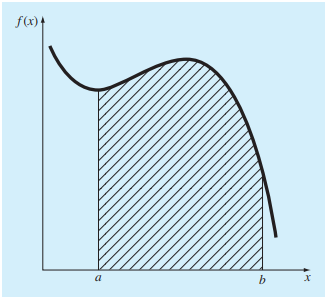
\includegraphics[scale=0.8]{fig_19_1}
   \caption{\textsf{Graphical representation of the integral of f (x) between the limits x = a to b. The integral is
   equivalent to the area under the curve.}}\label{fig:fig_19_1}
\end{figure}

\section{Integration in Engineering and Science}
Integration has so many engineering and scientific applications that you were required to
take integral calculus in your first year at college. Many specific examples of such applications could be given in all fields of engineering and science. A number of examples relate directly to the idea of the integral as the area under a curve. Figure 19.2 depicts a few
cases where integration is used for this purpose.\\

Other common applications relate to the analogy between integration and summation.
For example, a common application is to determine the mean of a continuous function.
Recall that the mean of n discrete data points can be calculated by [Eq. (14.2)].

\begin{equation}
    \tag{19.6}
	\operatorname{Mean}=\frac{\sum_{i=1}^{n} y_{i}}{n}
	\end{equation}

	where $y\textsubscript{i}$ are individual measurements. The determination of the mean of discrete points is
	depicted in Fig. 19.3a.

	In contrast, suppose that y is a continuous function of an independent variable x, as
	depicted in Fig. 19.3b. For this case, there are an infinite number of values between a and
	b. Just as Eq. (19.6) can be applied to determine the mean of the discrete readings,
	you might also be interested in computing the mean or average of the continuous function
	y = f (x) for the interval from a to b. Integration is used for this purpose, as specified by 

	\begin{equation}
		\tag{19.7}
		\operatorname{Mean}=\frac{\int_{a}^{b} f(x) d x}{b-a}
		\end{equation}

		This formula has hundreds of engineering and scientific applications. For example, it is
		used to calculate the center of gravity of irregular objects in mechanical and civil engineering and to determine the root-mean-square current in electrical engineering.

		\begin{figure}[H]
			\centering
			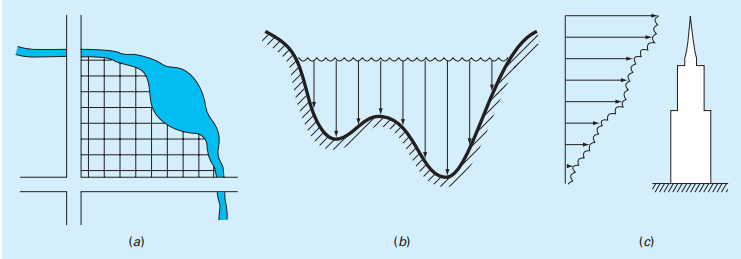
\includegraphics[scale=0.8]{fig_19_2}
		   \caption{\textsf{Examples of how integration is used to evaluate areas in engineering and scientific applications. (a) A surveyor might
		   need to know the area of a field bounded by a meandering stream and two roads. (b) A hydrologist might need to
		   know the cross-sectional area of a river. (c) A structural engineer might need to determine the net force due to a
		   nonuniform wind blowing against the side of a skyscraper.}}\label{fig:fig_19_2}
		\end{figure}

		\begin{figure}[H]
			\centering
			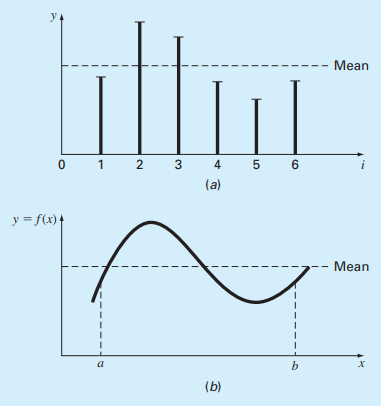
\includegraphics[scale=0.8]{fig_19_3}
		   \caption{\textsf{An illustration of the mean for (a) discrete and (b) continuous data}}\label{fig:fig_19_3}
		\end{figure}

		Integrals are also employed by engineers and scientists to evaluate the total amount or
		quantity of a given physical variable. The integral may be evaluated over a line, an area, or
		a volume. For example, the total mass of chemical contained in a reactor is given as the
		product of the concentration of chemical and the reactor volume, or
		$$
		\text { Mass }= \text { concentration } \times \text { volume }
		$$
		where concentration has units of mass per volume. However, suppose that concentration varies from location to location within the reactor. In this case, it is necessary to sum the products of local concentrations $c_{i}$ and corresponding elemental volumes $\Delta V_{i}$ :
		$$
		\text { Mass }=\sum_{i=1}^{n} c_{i} \Delta V_{i}
		$$
		where $n$ is the number of discrete volumes. For the continuous case, where $c(x, y, z)$ is a known function and $x, y$, and $z$ are independent variables designating position in Cartesian coordinates, integration can be used for the same purpose:
		$$
		\text { Mass }=\iiint c(x, y, z) d x d y d z
		$$
		or
		$$
		\text { Mass }=\iiint_{V} c(V) d V
		$$
		which is referred to as a volume integral. Notice the strong analogy between summation and integration.
		
		Similar examples could be given in other fields of engineering and science. For example, the total rate of energy transfer across a plane where the flux (in calories per square centimeter per second) is a function of position is given by
		$$
		\text { Flux }=\iint_{A} \text { ux } d A
		$$
		which is referred to as an areal integral, where A = area.\\
		These are just a few of the applications of integration that you might face regularly in
		the pursuit of your profession. When the functions to be analyzed are simple, you will normally choose to evaluate them analytically. However, it is often difficult or impossible
		when the function is complicated, as is typically the case in more realistic examples. In addition, the underlying function is often unknown and defined only by measurement at discrete points. For both these cases, you must have the ability to obtain approximate values
		for integrals using numerical techniques as described next.

		\section{NEWTON-COTES FORMULAS}
		The Newton-Cotes formulas are the most common numerical integration schemes. They
		are based on the strategy of replacing a complicated function or tabulated data with a polynomial that is easy to integrate:

		\begin{equation}
			\tag{19.8}
		I=\int_{a}^{b} f(x) d x \cong \int_{a}^{b} f_{n}(x) d x
	\end{equation}
		where $f_{n}(x)=$ a polynomial of the form
		\begin{equation}
			\tag{19.9}
		f_{n}(x)=a_{0}+a_{1} x+\cdots+a_{n-1} x^{n-1}+a_{n} x^{n}
	\end{equation}

	where n is the order of the polynomial. For example, in Fig. 19.4a, a first-order polynomial
	(a straight line) is used as an approximation. In Fig. 19.4b, a parabola is employed for the
	same purpose.\\
	The integral can also be approximated using a series of polynomials applied piecewise
	to the function or data over segments of constant length. For example, in Fig. 19.5, three

	\begin{figure}[H]
		\centering
		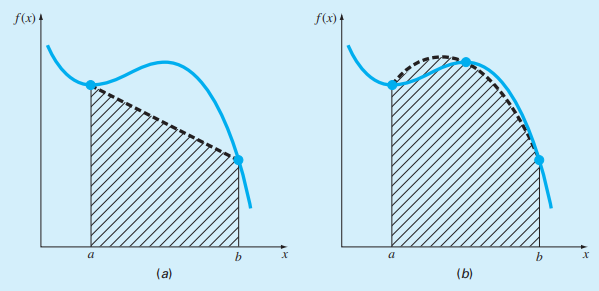
\includegraphics[scale=0.8]{fig_19_4}
	   \caption{\textsf{The approximation of an integral by the area under (a) a straight line and (b) a parabola.}}\label{fig:fig_19_4}
	\end{figure}
	\begin{figure}[H]
		\centering
		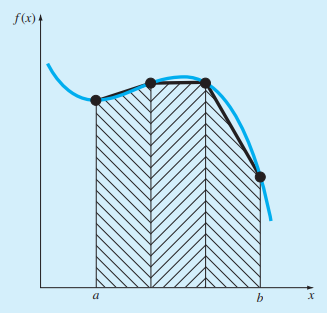
\includegraphics[scale=0.8]{fig_19_5}
	   \caption{\textsf{The approximation of an integral by the area under three straight-line segments}}\label{fig:fig_19_5}
	\end{figure}
	\begin{figure}[H]
		\centering
		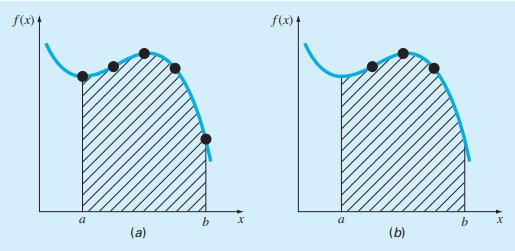
\includegraphics[scale=0.8]{fig_19_6}
	   \caption{\textsf{The difference between (a) closed and (b) open integration formulas}}\label{fig:fig_19_6}
	\end{figure}

	straight-line segments are used to approximate the integral. Higher-order polynomials can
	be utilized for the same purpose.\\
	Closed and open forms of the Newton-Cotes formulas are available. The closed forms
are those where the data points at the beginning and end of the limits of integration are
known (Fig. 19.6a). The open forms have integration limits that extend beyond the range
of the data (Fig. 19.6b). This chapter emphasizes the closed forms. However, material on
open Newton-Cotes formulas is briefly introduced in Section 19.7.
\vspace{1cm}
\section{THE TRAPEZOIDAL RULE}

The trapezoidal rule is the first of the Newton-Cotes closed integration formulas. It corresponds to the case where the polynomial in Eq. (19.8) is first-order:

\begin{equation}
    \tag{19.10}
I=\int_{a}^{b}\left[f(a)+\frac{f(b)-f(a)}{b-a}(x-a)\right] d x
\end{equation}
The result of the integration is
\begin{equation}
    \tag{19.11}
I=(b-a) \frac{f(a)+f(b)}{2}
\end{equation}
which is called the trapezoidal rule.
Geometrically, the trapezoidal rule is equivalent to approximating the area of the trapezoid under the straight line connecting $f(a)$ and $f(b)$ in Fig. 19.7. Recall from geometry that the formula for computing the area of a trapezoid is the height times the average of the bases. In our case, the concept is the same but the trapezoid is on its side. Therefore, the integral estimate can be represented as
\begin{equation}
    \tag{19.12}
I=\text { width } \times \text { average height }
\end{equation}

\begin{figure}[H]
    \centering
    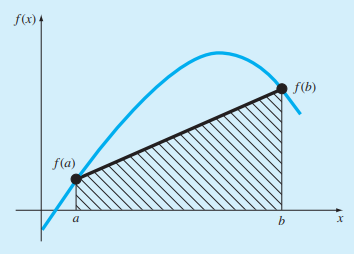
\includegraphics[scale=0.8]{fig_19_7}
   \caption{\textsf{Graphical depiction of the trapezoidal rule}}\label{fig:fig_19_7}
\end{figure}
or
\begin{equation}
    \tag{19.13}
	I=(b-a) \times \text { average height }
\end{equation}
where, for the trapezoidal rule, the average height is the average of the function values at the end points, or $[f(a)+f(b)] / 2$.

All the Newton-Cotes closed formulas can be expressed in the general format of Eq. (19.13). That is, they differ only with respect to the formulation of the average height.
\subsection{Error of the Trapezoidal Rule}
When we employ the integral under a straight-line segment to approximate the integral under a curve, we obviously can incur an error that may be substantial (Fig. 19.8). An estimate for the local truncation error of a single application of the trapezoidal rule is
\begin{equation}
    \tag{19.14}
E_{t}=-\frac{1}{12} f^{\prime \prime}(\xi)(b-a)^{3}
\end{equation}
where $\xi$ lies somewhere in the interval from $a$ to $b$. Equation (19.14) indicates that if the function being integrated is linear, the trapezoidal rule will be exact because the second derivative of a straight line is zero. Otherwise, for functions with second- and higher-order derivatives (i.e., with curvature), some error can occur.

\begin{exmp} \textbf{Single Application of the Trapezoidal Rule}
    \noindent\textit{Problem Statement.} Use Eq. (19.11) to numerically integrate
    \begin{equation}
		f(x)=0.2+25 x-200 x^{2}+675 x^{3}-900 x^{4}+400 x^{5}\nonumber
		\end{equation}
		from a = 0 to b = 0.8. Note that the exact value of the integral can be determined analytically to be 1.640533.

		\begin{figure}[H]
			\centering
			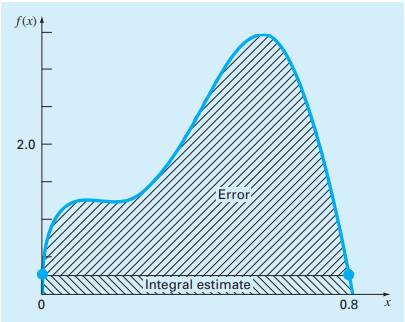
\includegraphics[scale=0.8]{fig_19_8}
		   \caption{\textsf{Graphical depiction of the use of a single application of the trapezoidal rule to approximate the integral of $f(x)=0.2+25 x-200 x^{2}+675 x^{3}-900 x^{4}+400 x^{5}$ from $x=0$ to $0.8$.}}\label{fig:fig_19_8}
		\end{figure}

	\noindent \textbf{Solution.} The function values f (0) = 0.2 and f (0.8) = 0.232 can be substituted into
	Eq. (19.11) to yield
	$$
I=(0.8-0) \frac{0.2+0.232}{2}=0.1728
$$
which represents an error of $E_{t}=1.640533-0.1728=1.467733$, which corresponds to a percent relative error of $\varepsilon_{t}=89.5 \%$. The reason for this large error is evident from the graphical depiction in Fig. 19.8. Notice that the area under the straight line neglects a significant portion of the integral lying above the line.

In actual situations, we would have no foreknowledge of the true value. Therefore, an approximate error estimate is required. To obtain this estimate, the function's second derivative over the interval can be computed by differentiating the original function twice to give
$$
f^{\prime \prime}(x)=-400+4,050 x-10,800 x^{2}+8,000 x^{3}
$$
The average value of the second derivative can be computed as [Eq. (19.7)]
$$
\bar{f}^{\prime \prime}(x)=\frac{\int_{0}^{0.8}\left(-400+4,050 x-10,800 x^{2}+8,000 x^{3}\right) d x}{0.8-0}=-60
$$
which can be substituted into Eq. (19.14) to yield
$$
E_{a}=-\frac{1}{12}(-60)(0.8)^{3}=2.56
$$
which is of the same order of magnitude and sign as the true error. A discrepancy does exist, however, because of the fact that for an interval of this size, the average second derivative is not necessarily an accurate approximation of $f^{\prime \prime}(\xi)$. Thus, we denote that the error is approximate by using the notation $E_{a}$, rather than exact by using $E_{t}$.
\end{exmp}

\subsection{The Composite Trapezoidal Rule}

One way to improve the accuracy of the trapezoidal rule is to divide the integration interval
from a to b into a number of segments and apply the method to each segment (Fig. 19.9).
The areas of individual segments can then be added to yield the integral for the entire
interval. The resulting equations are called composite, or multiple-segment, integration
formulas\\
Figure 19.9 shows the general format and nomenclature we will use to characterize
composite integrals. There are n + 1 equally spaced base points ($x\textsubscript{0}$, $x\textsubscript{1}$, $x\textsubscript{2}$,..., $x\textsubscript{n}$). Consequently, there are n segments of equal width:

\begin{equation}
    \tag{19.15}
h=\frac{b-a}{n}
\end{equation}
If $a$ and $b$ are designated as $x_{0}$ and $x_{n}$, respectively, the total integral can be represented as
\begin{equation}
I=\int_{x_{0}}^{x_{1}} f(x) d x+\int_{x_{1}}^{x_{2}} f(x) d x+\cdots+\int_{x_{n-1}}^{x_{n}} f(x) d x
\nonumber\end{equation}

\begin{figure}[H]
    \centering
    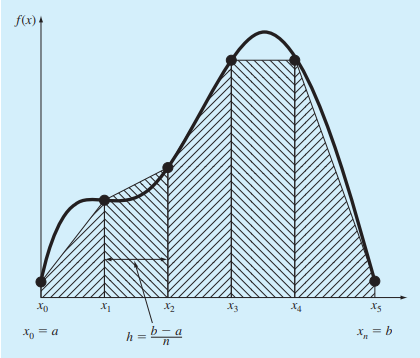
\includegraphics[scale=0.6]{fig_19_9}
   \caption{\textsf{Composite trapezoidal rule.}}\label{fig:fig_19_9}
\end{figure}

Substituting the trapezoidal rule for each integral yields

\begin{equation}
    \tag{19.16}
I=h \frac{f\left(x_{0}\right)+f\left(x_{1}\right)}{2}+h \frac{f\left(x_{1}\right)+f\left(x_{2}\right)}{2}+\cdots+h \frac{f\left(x_{n-1}\right)+f\left(x_{n}\right)}{2}
\end{equation}
or, grouping terms:
\begin{equation}
    \tag{19.17}
I=\frac{h}{2}\left[f\left(x_{0}\right)+2 \sum_{i=1}^{n-1} f\left(x_{i}\right)+f\left(x_{n}\right)\right]
\end{equation}
or, using Eq. (19.15) to express Eq. (19.17) in the general form of Eq. (19.13):
\begin{equation}
    \tag{19.18}
I=\underbrace{(b-a)}_{\text {Width }} \underbrace{\frac{f\left(x_{0}\right)+2 \sum_{i=1}^{n-1} f\left(x_{i}\right)+f\left(x_{n}\right)}{2 n}}_{\text {Average height }}
\end{equation}
Because the summation of the coefficients of $f(x)$ in the numerator divided by $2 n$ is equal to 1 , the average height represents a weighted average of the function values. According to Eq. (19.18), the interior points are given twice the weight of the two end points $f\left(x_{0}\right)$ and $f\left(x_{n}\right)$.

An error for the composite trapezoidal rule can be obtained by summing the individual errors for each segment to give
\begin{equation}
    \tag{19.19}
E_{t}=-\frac{(b-a)^{3}}{12 n^{3}} \sum_{i=1}^{n} f^{\prime \prime}\left(\xi_{i}\right)
\end{equation}
where $f^{\prime \prime}\left(\xi_{i}\right)$ is the second derivative at a point $\xi_{i}$ located in segment $i$. This result can be simplified by estimating the mean or average value of the second derivative for the entire interval as
\begin{equation}
    \tag{19.20}
\overline{f^{\prime \prime}} \cong \frac{\sum_{i=1}^{n} f^{\prime \prime}\left(\xi_{i}\right)}{n}
\end{equation}
Therefore $\sum f^{\prime \prime}\left(\xi_{i}\right) \cong n \bar{f}^{\prime \prime}$ and Eq. (19.19) can be rewritten as
\begin{equation}
    \tag{19.21}
E_{a}=-\frac{(b-a)^{3}}{12 n^{2}} \bar{f}^{\prime \prime}
\end{equation}
Thus, if the number of segments is doubled, the truncation error will be quartered. Note that Eq. (19.21) is an approximate error because of the approximate nature of Eq. (19.20).

\begin{exmp} \textbf{Composite Application of the Trapezoidal Rule}
    \noindent\textit{Problem Statement.}Use the two-segment trapezoidal rule to estimate the integral of
    
	$$
f(x)=0.2+25 x-200 x^{2}+675 x^{3}-900 x^{4}+400 x^{5}
$$
from $a=0$ to $b=0.8$. Employ Eq. (19.21) to estimate the error. Recall that the exact value of the integral is $1.640533$.
	
	\noindent \textbf{Solution.}
	For $n=2(h=0.4)$ :
$$
\begin{aligned}
f(0) &=0.2 \quad f(0.4)=2.456 \quad f(0.8)=0.232 \\
I &=0.8 \frac{0.2+2(2.456)+0.232}{4}=1.0688 \\
E_{t} &=1.640533-1.0688=0.57173 \quad \varepsilon_{t}=34.9 \% \\
E_{a} &=-\frac{0.8^{3}}{12(2)^{2}}(-60)=0.64
\end{aligned}
$$
where $-60$ is the average second derivative determined previously in Example 19.1.
	
\end{exmp}
The results of the previous example, along with three- through ten-segment applications of the trapezoidal rule, are summarized in Table 19.1. Notice how the error decreases
as the number of segments increases. However, also notice that the rate of decrease is gradual. This is because the error is inversely related to the square of n [Eq. (19.21)]. Therefore,
doubling the number of segments quarters the error. In subsequent sections we develop
higher-order formulas that are more accurate and that converge more quickly on the true integral as the segments are increased. However, before investigating these formulas, we will
first discuss how MATLAB can be used to implement the trapezoidal rule.

\subsection{MATLAB M-file: trap}

A simple algorithm to implement the composite trapezoidal rule can be written as in
Fig. 19.10. The function to be integrated is passed into the M-file along with the limits of
integration and the number of segments. A loop is then employed to generate the integral
following Eq. (19.18).
\textit{TABLE 19.1} Results for the composite trapezoidal rule to estimate the integral of $f(x)=0.2+25 x-$ $200 x^{2}+675 x^{3}-900 x^{4}+400 x^{5}$ from $x=0$ to $0.8$. The exact value is $1.640533$.
\begin{center}
\begin{tabular}{rlrr}
\hline $\boldsymbol{n}$ & \multicolumn{1}{c}{$\boldsymbol{h}$} & \multicolumn{1}{c}{$\boldsymbol{I}$} & $\boldsymbol{\varepsilon}_{\boldsymbol{t}}(\%)$ \\
\hline 2 & $0.4$ & $1.0688$ & $34.9$ \\
3 & $0.2667$ & $1.3695$ & $16.5$ \\
4 & $0.2$ & $1.4848$ & $9.5$ \\
5 & $0.16$ & $1.5399$ & $6.1$ \\
6 & $0.1333$ & $1.5703$ & $4.3$ \\
7 & $0.1143$ & $1.5887$ & $3.2$ \\
8 & $0.1$ & $1.6008$ & $2.4$ \\
9 & $0.0889$ & $1.6091$ & $1.9$ \\
10 & $0.08$ & $1.6150$ & $1.6$ \\
\hline
\end{tabular}
\end{center}

\begin{lstlisting}[numbers=none]
	function I = trap(func,a,b,n,varargin)
	% trap: composite trapezoidal rule quadrature
	% I = trap(func,a,b,n,pl,p2,...):
	% composite trapezoidal rule
	% input:
	% func = name of function to be integrated
	% a, b = integration limits
	% n = number of segments (default = 100)
	% pl,p2,... = additional parameters used by func
	% output:
	% I = integral estimate
	if nargin<3,error('at least 3 input arguments required'),end
	if ~(b>a),error('upper bound must be greater than lower'),end
	if nargin<4|isempty(n),n=100;end
	x = a; h = (b - a)/n;
	s=func(a,varargin{:});
	for i = 1 : n-1
	x = x + h;
	s = s + 2*func(x,varargin{:});
	end
	s = s + func(b,varargin{:});
	I = (b - a) * s/(2*n);
\end{lstlisting}
\begin{figure}[H]
    \centering
    
\includegraphics[scale=0.6]{fig_19_10}
   \caption{\textsf{M-file to implement the composite trapezoidal rule}}\label{fig:fig_19_10}
\end{figure}
An application of the M-file can be developed to determine the distance fallen by the free-falling bungee jumper in the first $3 \mathrm{~s}$ by evaluating the integral of Eq. (19.3). For this example, assume the following parameter values: $g=9.81 \mathrm{~m} / \mathrm{s}^{2}, m=68.1 \mathrm{~kg}$, and $c_{d}=0.25 \mathrm{~kg} / \mathrm{m}$. Note that the exact value of the integral can be computed with Eq. (19.4) as $41.94805$.
The function to be integrated can be developed as an M-file or with an anonymous
function,

\begin{lstlisting}[numbers=none]
>> v=@(t) sqrt(9.81*68.1/0.25)*tanh(sqrt(9.81*0.25/68.1)*t)
v =
@(t) sqrt(9.81*68.1/0.25)*tanh(sqrt(9.81*0.25/68.1)*t)
\end{lstlisting}

First, let's evaluate the integral with a crude five-segment approximation:

\begin{lstlisting}[numbers=none]
	format long
	>> trap(v,0,3,5)
	ans =
	41.86992959072735
\end{lstlisting}

As would be expected, this result has a relatively high true error of 18.6\%{}. To obtain a more
accurate result, we can use a very fine approximation based on 10,000 segments:

\begin{lstlisting}[numbers=none]
>> trap(v,0,3,10000)
x =
	41.94804999917528
\end{lstlisting}
which is very close to the true value.

\section{SIMPSON'S RULES}
Aside from applying the trapezoidal rule with finer segmentation, another way to obtain a
more accurate estimate of an integral is to use higher-order polynomials to connect the
points. For example, if there is an extra point midway between f (a) and f (b), the three
points can be connected with a parabola (Fig. 19.11a). If there are two points equally
spaced between f (a) and f (b), the four points can be connected with a third-order polynomial (Fig. 19.11b). The formulas that result from taking the integrals under these polynomials are called Simpson's rules.

\subsection{Simpson's 1/3 Rule}

Simpson's 1/3 rule corresponds to the case where the polynomial in Eq. (19.8) is secondorder:

\begin{equation}
	\begin{aligned}
	I=& \int_{x_{0}}^{x_{2}}\left[\frac{\left(x-x_{1}\right)\left(x-x_{2}\right)}{\left(x_{0}-x_{1}\right)\left(x_{0}-x_{2}\right)} f\left(x_{0}\right)+\frac{\left(x-x_{0}\right)\left(x-x_{2}\right)}{\left(x_{1}-x_{0}\right)\left(x_{1}-x_{2}\right)} f\left(x_{1}\right)\right.\\
	&\left.+\frac{\left(x-x_{0}\right)\left(x-x_{1}\right)}{\left(x_{2}-x_{0}\right)\left(x_{2}-x_{1}\right)} f\left(x_{2}\right)\right] d x
	\end{aligned} \nonumber
	\end{equation}

	\begin{figure}[H]
		\centering
		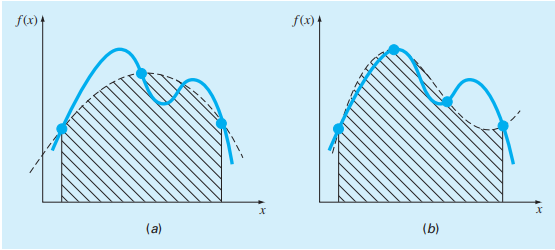
\includegraphics[scale=0.8]{fig_19_11}
	   \caption{\textsf{(a) Graphical depiction of Simpson's 1/3 rule: It consists of taking the area under a parabola
	   connecting three points. (b) Graphical depiction of Simpson's 3/8 rule: It consists of taking the
	   area under a cubic equation connecting four points.}}\label{fig:fig_19_11}
	\end{figure}
	where a and b are designated as $x\textsubscript{0}$ and $x\textsubscript{2}$, respectively. The result of the integration is

	\begin{equation}
		\tag{19.22}
	I=\frac{h}{3}\left[f\left(x_{0}\right)+4 f\left(x_{1}\right)+f\left(x_{2}\right)\right]
\end{equation}
	where, for this case, $h=(b-a) / 2$. This equation is known as Simpson's $1 / 3$ rule. The label " $1 / 3$ " stems from the fact that $h$ is divided by 3 in Eq. (19.22). Simpson's $1 / 3$ rule can also be expressed using the format of Eq. (19.13):
	\begin{equation}
		\tag{19.23}
	I=(b-a) \frac{f\left(x_{0}\right)+4 f\left(x_{1}\right)+f\left(x_{2}\right)}{6}
\end{equation}
	where $a=x_{0}, b=x_{2}$, and $x_{1}=$ the point midway between $a$ and $b$, which is given by $(a+b) / 2$. Notice that, according to Eq. (19.23), the middle point is weighted by twothirds and the two end points by one-sixth.
	
	It can be shown that a single-segment application of Simpson's $1 / 3$ rule has a truncation error of
	$$
	E_{t}=-\frac{1}{90} h^{5} f^{(4)}(\xi)
	$$
	or, because $h=(b-a) / 2$ :
	\begin{equation}
		\tag{19.24}
	E_{t}=-\frac{(b-a)^{5}}{2880} f^{(4)}(\xi)
\end{equation}
	where $\xi$ lies somewhere in the interval from $a$ to $b$. Thus, Simpson's $1 / 3$ rule is more accurate than the trapezoidal rule. However, comparison with Eq. (19.14) indicates that it is more accurate than expected. Rather than being proportional to the third derivative, the error is proportional to the fourth derivative. Consequently, Simpson's $1 / 3$ rule is thirdorder accurate even though it is based on only three points. In other words, it yields exact results for cubic polynomials even though it is derived from a parabola!

	\begin{exmp} \textbf{Single Application of Simpson's 1/3 Rule}
		\noindent\textit{Problem Statement.} Use Eq. (19.23) to integrate
		$$
f(x)=0.2+25 x-200 x^{2}+675 x^{3}-900 x^{4}+400 x^{5}
$$
from $a=0$ to $b=0.8$. Employ Eq. (19.24) to estimate the error. Recall that the exact integral is $1.640533$.

		\noindent \textbf{Solution.}$\quad n=2(h=0.4)$ :
		$$
		\begin{aligned}
		f(0) &=0.2 \quad f(0.4)=2.456 \quad f(0.8)=0.232 \\
		I &=0.8 \frac{0.2+4(2.456)+0.232}{6}=1.367467 \\
		E_{t} &=1.640533-1.367467=0.2730667 \quad \varepsilon_{t}=16.6 \%
		\end{aligned}
		$$
		which is approximately five times more accurate than for a single application of the trapezoidal rule (Example 19.1). The approximate error can be estimated as
		$$
		E_{a}=-\frac{0.8^{5}}{2880}(-2400)=0.2730667
		$$
		where $-2400$ is the average fourth derivative for the interval. As was the case in Example $19.1$, the error is approximate $\left(E_{a}\right)$ because the average fourth derivative is generally not an exact estimate of $f^{(4)}(\xi)$. However, because this case deals with a fifth-order polynomial, the result matches exactly.
	\end{exmp}

	\subsection{The Composite Simpson's 1/3 Rule}
	Just as with the trapezoidal rule, Simpson's rule can be improved by dividing the integration interval into a number of segments of equal width (Fig. 19.12). The total integral can
	be represented as

	\begin{equation}
		\tag{19.25}
		I=\int_{x_{0}}^{x_{2}} f(x) d x+\int_{x_{2}}^{x_{4}} f(x) d x+\cdots+\int_{x_{n-2}}^{x_{n}} f(x) d x
		\end{equation}

		\begin{figure}[H]
			\centering
			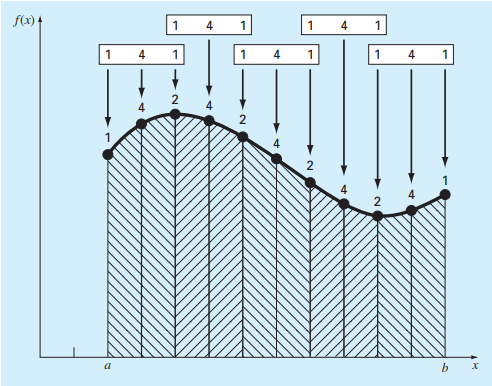
\includegraphics[scale=0.8]{fig_19_12}
		   \caption{\textsf{Composite Simpson's 1/3 rule. The relative weights are depicted above the function values.
		   Note that the method can be employed only if the number of segments is even.}}\label{fig:fig_19_12}
		\end{figure}


		Substituting Simpson's $1 / 3$ rule for each integral yields
		$$
		\begin{aligned}
		I=& 2 h \frac{f\left(x_{0}\right)+4 f\left(x_{1}\right)+f\left(x_{2}\right)}{6}+2 h \frac{f\left(x_{2}\right)+4 f\left(x_{3}\right)+f\left(x_{4}\right)}{6} \\
		&+\cdots+2 h \frac{f\left(x_{n-2}\right)+4 f\left(x_{n-1}\right)+f\left(x_{n}\right)}{6}
		\end{aligned}
		$$
		or, grouping terms and using Eq. (19.15):
		\begin{equation}
			\tag{19.26}
		I=(b-a) \frac{f\left(x_{0}\right)+4 \sum_{i=1,3,5}^{n-1} f\left(x_{i}\right)+2 \sum_{j=2,4,6}^{n-2} f\left(x_{j}\right)+f\left(x_{n}\right)}{3 n}
	\end{equation}
		Notice that, as illustrated in Fig. 19.12, an even number of segments must be utilized to implement the method. In addition, the coefficients "4" and " 2 " in Eq. (19.26) might seem peculiar at first glance. However, they follow naturally from Simpson's $1 / 3$ rule. As illustrated in Fig. 19.12, the odd points represent the middle term for each application and hence carry the weight of four from Eq. (19.23). The even points are common to adjacent applications and hence are counted twice.
		
		An error estimate for the composite Simpson's rule is obtained in the same fashion as for the trapezoidal rule by summing the individual errors for the segments and averaging the derivative to yield
		\begin{equation}
			\tag{19.27}
		E_{a}=-\frac{(b-a)^{5}}{180 n^{4}} \bar{f}^{(4)}
	\end{equation}
		where $f^{(4)}$ is the average fourth derivative for the interval.

		\begin{exmp} \textbf{Composite Simpson's 1/3 Rule}
			\noindent\textit{Problem Statement.}Use Eq. (19.26) with n = 4 to estimate the integral of
			$$
f(x)=0.2+25 x-200 x^{2}+675 x^{3}-900 x^{4}+400 x^{5}
$$
from $a=0$ to $b=0.8$. Employ Eq. (19.27) to estimate the error. Recall that the exact integral is $1.640533$.

			\noindent \textbf{Solution.}$n=4(h=0.2)$ :
			$$
			\begin{aligned}
			f(0) &=0.2 & & f(0.2)=1.288 \\
			f(0.4) &=2.456 & & f(0.6)=3.464 \\
			f(0.8) &=0.232 & &
			\end{aligned}
			$$
			From Eq. (19.26):
			$$
			\begin{aligned}
			I &=0.8 \frac{0.2+4(1.288+3.464)+2(2.456)+0.232}{12}=1.623467 \\
			E_{t} &=1.640533-1.623467=0.017067 \quad \varepsilon_{t}=1.04 \%
			\end{aligned}
			$$
			The estimated error (Eq. 19.27) is
			$$
			E_{a}=-\frac{(0.8)^{5}}{180(4)^{4}}(-2400)=0.017067
			$$
			which is exact (as was also the case for Example 19.3).
		\end{exmp}
		As in Example 19.4, the composite version of Simpson's 1/3 rule is considered superior to the trapezoidal rule for most applications. However, as mentioned previously, it is
		limited to cases where the values are equispaced. Further, it is limited to situations where
		there are an even number of segments and an odd number of points. Consequently, as discussed in Section 19.4.3, an odd-segment-even-point formula known as Simpson's 3/8
		rule can be used in conjunction with the 1/3 rule to permit evaluation of both even and odd
		numbers of equispaced segments.

		\subsection{ Simpson's 3/8 Rule}

		In a similar manner to the derivation of the trapezoidal and Simpson’s 1/3 rule, a thirdorder Lagrange polynomial can be fit to four points and integrated to yield

		$$
I=\frac{3 h}{8}\left[f\left(x_{0}\right)+3 f\left(x_{1}\right)+3 f\left(x_{2}\right)+f\left(x_{3}\right)\right]
$$
where $h=(b-a) / 3$. This equation is known as Simpsons $3 / 8$ rule because $h$ is multiplied by $3 / 8$. It is the third Newton-Cotes closed integration formula. The $3 / 8$ rule can also be expressed in the form of Eq. (19.13):
\begin{equation}
    \tag{19.28}
I=(b-a) \frac{f\left(x_{0}\right)+3 f\left(x_{1}\right)+3 f\left(x_{2}\right)+f\left(x_{3}\right)}{8}
\end{equation}
Thus, the two interior points are given weights of three-eighths, whereas the end points are weighted with one-eighth. Simpson's $3 / 8$ rule has an error of
$$
E_{t}=-\frac{3}{80} h^{5} f^{(4)}(\xi)
$$
or, because $h=(b-a) / 3$ :
\begin{equation}
    \tag{19.29}
E_{t}=-\frac{(b-a)^{5}}{6480} f^{(4)}(\xi)
\end{equation}

Because the denominator of Eq. (19.29) is larger than for Eq. (19.24), the 3/8 rule is somewhat more accurate than the 1/3 rule.\\

Simpson's 1/3 rule is usually the method of preference because it attains third-order
accuracy with three points rather than the four points required for the 3/8 version. However, the 3/8 rule has utility when the number of segments is odd. For instance, in Example 19.4 we used Simpson's rule to integrate the function for four segments. Suppose that
you desired an estimate for five segments. One option would be to use a composite version
of the trapezoidal rule as was done in Example 19.2. This may not be advisable, however,
because of the large truncation error associated with this method. An alternative would be
to apply Simpson's 1/3 rule to the first two segments and Simpson's 3/8 rule to the last

\begin{figure}[H]
    \centering
    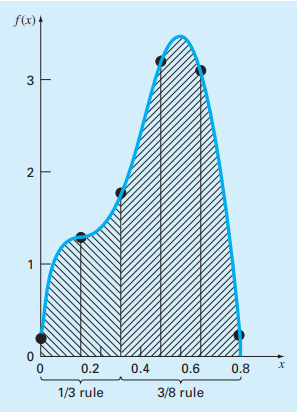
\includegraphics[scale=0.8]{fig_19_13}
   \caption{\textsf{Illustration of how Simpson's 1/3 and 3/8 rules can be applied in tandem to handle multiple
   applications with odd numbers of intervals.}}\label{fig:fig_19_13}
\end{figure}
three (Fig. 19.13). In this way, we could obtain an estimate with third-order accuracy across
the entire interval.

\begin{exmp} \textbf{Simpson's 3/8 Rule}
    \noindent\textit{Problem Statement.}(a) Use Simpson's 3/8 rule to integrate
    $$
f(x)=0.2+25 x-200 x^{2}+675 x^{3}-900 x^{4}+400 x^{5}
$$
from $a=0$ to $b=0.8$. ( $b$ ) Use it in conjunction with Simpson's $1 / 3$ rule to integrate the same function for five segments.


	\noindent \textbf{Solution.} (a) A single application of Simpson's $3 / 8$ rule requires four equally spaced points:
	$$
	\begin{array}{ll}
	f(0)=0.2 & f(0.2667)=1.432724 \\
	f(0.5333)=3.487177 & f(0.8)=0.232
	\end{array}
	$$
	Using Eq. (19.28):
	$$
	I=0.8 \frac{0.2+3(1.432724+3.487177)+0.232}{8}=1.51970
	$$
	(b) The data needed for a five-segment application $(h=0.16)$ are
	$$
	\begin{array}{ll}
	f(0)=0.2 & f(0.16)=1.296919 \\
	f(0.32)=1.743393 & f(0.48)=3.186015 \\
	f(0.64)=3.181929 & f(0.80)=0.232
	\end{array}
	$$
	The integral for the first two segments is obtained using Simpson's $1 / 3$ rule:
	$$
	I=0.32 \frac{0.2+4(1.296919)+1.743393}{6}=0.3803237
	$$
	For the last three segments, the $3 / 8$ rule can be used to obtain
	$$
	I=0.48 \frac{1.743393+3(3.186015+3.181929)+0.232}{8}=1.264754
	$$
	The total integral is computed by summing the two results:
	$$
	I=0.3803237+1.264754=1.645077
	$$
\end{exmp}

\section{ HIGHER-ORDER NEWTON-COTES FORMULAS}
As noted previously, the trapezoidal rule and both of Simpson's rules are members of a
family of integrating equations known as the Newton-Cotes closed integration formulas.
Some of the formulas are summarized in Table 19.2 along with their truncation-error
estimates.\\
Notice that, as was the case with Simpson's 1/3 and 3/8 rules, the five- and six-point
formulas have the same order error. This general characteristic holds for the higher-point
formulas and leads to the result that the even-segment-odd-point formulas (e.g., 1/3 rule
and Boole's rule) are usually the methods of preference.
\\\textit{TABLE 19.2} Newton-Cotes closed integration formulas. The formulas are presented in the format of Eq. (19.13) so that the weighting of the data points to estimate the average height is apparent. The step size is given by $h=(b-a) / n$.
$$
\begin{aligned}
&\text { Segments }\\
&\begin{array}{cclll}
\text { (n) } & \text { Points } & \text { Name } & \text { Formula } & \text { Trunction Error } \\
\hline 1 & 2 & \text { Trapezoidal rule } &(b-a) \frac{f\left(x_{0}\right)+f\left(x_{1}\right)}{2} &-(1 / 12) h^{3} f^{\prime \prime}(\xi)\\
2 & 3 & \text { Simpson's } 1 / 3 \text { rule } &(b-a) \frac{f\left(x_{0}\right)+4 f\left(x_{1}\right)+f\left(x_{2}\right)}{6} &-(1 / 90) h^{5} f^{(4)}(\xi)\\
3 & 4 & \text { Simpson's } 3 / 8 \text { rule } &(b-a) \frac{f\left(x_{0}\right)+3 f\left(x_{1}\right)+3 f\left(x_{2}\right)+f\left(x_{3}\right)}{8} &-\left(3 / 80 \mid h^{5} f^{(4)}(\xi)\right.\\
4 & 5 & \text { Boole's rule } &(b-a) \frac{7 f\left(x_{0}\right)+32 f\left(x_{1}\right)+12 f\left(x_{2}\right)+32 f\left(x_{3}\right)+7 f\left(x_{4}\right)}{90} &-(8 / 945) h^{7} f^{(6)}(\xi)\\
5 & 6 & &(b-a) \frac{19 f\left(x_{0}\right)+75 f\left(x_{1}\right)+50 f\left(x_{2}\right)+50 f\left(x_{3}\right)+75 f\left(x_{4}\right)+19 f\left(x_{5}\right)}{288} &-(275 / 12,096) h^{7} f^{(6)}(\xi)\\
\hline
\end{array}
\end{aligned}
$$
However, it must also be stressed that, in engineering and science practice, the higherorder (i.e., greater than four-point) formulas are not commonly used. Simpson's rules are
sufficient for most applications. Accuracy can be improved by using the composite version.
Furthermore, when the function is known and high accuracy is required, methods such as
Romberg integration or Gauss quadrature, described in Chap. 20, offer viable and attractive alternatives.
\vspace{1cm}
\section{INTEGRATION WITH UNEQUAL SEGMENTS}
To this point, all formulas for numerical integration have been based on equispaced data
points. In practice, there are many situations where this assumption does not hold and we
must deal with unequal-sized segments. For example, experimentally derived data are
often of this type. For these cases, one method is to apply the trapezoidal rule to each segment and sum the results:
\begin{equation}
    \tag{19.30}
I=h_{1} \frac{f\left(x_{0}\right)+f\left(x_{1}\right)}{2}+h_{2} \frac{f\left(x_{1}\right)+f\left(x_{2}\right)}{2}+\cdots+h_{n} \frac{f\left(x_{n-1}\right)+f\left(x_{n}\right)}{2}
\end{equation}
where $h_{i}=$ the width of segment $i$. Note that this was the same approach used for the composite trapezoidal rule. The only difference between Eqs. (19.16) and (19.30) is that the $h$ 's in the former are constant.

\begin{exmp} \textbf{Trapezoidal Rule with Unequal Segments}
    \noindent\textit{Problem Statement.}The information in Table 19.3 was generated using the same polynomial employed in Example 19.1. Use Eq. (19.30) to determine the integral for these data.
	Recall that the correct answer is 1.640533.	

	\textit{TABLE 19.3} Data for $f(x)=0.2+25 x-200 x^{2}+675 x^{3}-900 x^{4}+400 x^{5}$, with unequally spaced values of $x$.\\
	\begin{center}
\begin{tabular}{cccc}
\hline $\boldsymbol{x}$ & $\boldsymbol{f}(\boldsymbol{x} \boldsymbol{)}$ & $\boldsymbol{x}$ & $\boldsymbol{f}(\boldsymbol{x} \boldsymbol{)}$ \\
\hline $0.00$ & $0.200000$ & $0.44$ & $2.842985$ \\
$0.12$ & $1.309729$ & $0.54$ & $3.507297$ \\
$0.22$ & $1.305241$ & $0.64$ & $3.181929$ \\
$0.32$ & $1.743393$ & $0.70$ & $2.363000$ \\
$0.36$ & $2.074903$ & $0.80$ & $0.232000$ \\
$0.40$ & $2.456000$ & & \\
\hline
\end{tabular}
\end{center}
    \noindent \textbf{Solution.} Applying Eq. (19.30) yields
	$$
	\begin{aligned}
	I=& 0.12 \frac{0.2+1.309729}{2}+0.10 \frac{1.309729+1.305241}{2} \\
	&+\cdots+0.10 \frac{2.363+0.232}{2}=1.594801
	\end{aligned}
	$$
	which represents an absolute percent relative error of $\varepsilon_{t}=2.8 \%$.
\end{exmp}

\subsection{MATLAB M-file: trapuneq}
A simple algorithm to implement the trapezoidal rule for unequally spaced data can be
written as in Fig. 19.14. Two vectors, x and y, holding the independent and dependent variables are passed into the M-file. Two error traps are included to ensure that (a) the two vectors are of the same length and (b) the x's are in ascending order.1 A loop is employed to
generate the integral. Notice that we have modified the subscripts from those of Eq. (19.30)
to account for the fact that MATLAB does not allow zero subscripts in arrays.
An application of the M-file can be developed for the same problem that was solved in
Example 19.6:
\begin{lstlisting}[numbers=none]
	>> x = [0 .12 .22 .32 .36 .4 .44 .54 .64 .7 .8];
	>> y = 0.2+25*x-200*x.^2+675*x.^3-900*x.^4+400*x.^5;
	>> trapuneq(x,y)
	ans =
		1.5948
\end{lstlisting}
which is identical to the result obtained in Example 19.6.

\begin{figure}[H]
    \centering
    
\includegraphics[scale=0.8]{fig_19_14}
   \caption{\textsf{M-file to implement the trapezoidal rule for unequally spaced data.}}\label{fig:fig_19_14}
\end{figure}

\begin{lstlisting}[numbers=none]
function I = trapuneq(x,y)
% trapuneq: unequal spaced trapezoidal rule quadrature
% I = trapuneq(x,y):
% Applies the trapezoidal rule to determine the integral
% for n data points (x, y) where x and y must be of the
% same length and x must be monotonically ascending
% input:
% x = vector of independent variables
% y = vector of dependent variables
% output:
% I = integral estimate
if nargin<2,error('at least 2 input arguments required'),end
if any(diff(x)<0),error('x not monotonically ascending'),end
n = length(x);
if length(y)~=n,error('x and y must be same length'); end
s = 0;
for k = 1:n-1
s = s + (x(k+l)-x(k))*(y(k)+y(k+l))/2;
end
I = s; 
\end{lstlisting}
The diff function is described in Section 21.7.1.

\subsection{ MATLAB Functions: trapz and cumtrapz}

MATLAB has a built-in function that evaluates integrals for data in the same fashion as the
M-file we just presented in Fig. 19.14. It has the general syntax 

\begin{lstlisting}[numbers=none]
	z = trapz(x, y)
\end{lstlisting}
where the two vectors, x and y, hold the independent and dependent variables, respectively.
Here is a simple MATLAB session that uses this function to integrate the data from
Table 19.3:

\begin{lstlisting}[numbers=none]
	>> x = [0 .12 .22 .32 .36 .4 .44 .54 .64.7 .8];
	>> y = 0.2+25*x-200*x.^2+675*x.^3-900*x.^4+400*x.^5;
	>> trapz(x,y)
	ans =
		1.5948
\end{lstlisting}
In addition, MATLAB has another function, cumtrapz, that computes the cumulative
integral. A simple representation of its syntax is 

\begin{lstlisting}[numbers=none]
	z = cumtrapz(x, y)
\end{lstlisting}
where the two vectors, x and y, hold the independent and dependent variables, respectively,
and z = a vector whose elements z(k) hold the integral from x(1) to x(k).

\begin{exmp} \textbf{Using Numerical Integration to Compute Distance from Velocity}
    \noindent\textit{Problem Statement.} As described at the beginning of this chapter, a nice application
	of integration is to compute the distance z(t) of an object based on its velocity v(t) as in
	(recall Eq. 19.2):
$$z(t)=\int_{0}^{t} v(t) d t$$
	Suppose that we had measurements of velocity at a series of discrete unequally spaced times
during free fall. Use Eq. (19.2) to synthetically generate such information for a 70-kg
jumper with a drag coefficient of 0.275 kg/m. Incorporate some random error by rounding
the velocities to the nearest integer. Then use cumtrapz to determine the distance fallen and
compare the results to the analytical solution (Eq. 19.4). In addition, develop a plot of the
analytical and computed distances along with velocity on the same graph.\\
    \noindent \textbf{Solution.}Some unequally spaced times and rounded velocities can be generated as
	\begin{lstlisting}[numbers=none]
>> format short g
>> t=[0 1 1.4 2 3 4.3 6 6.7 8];
>> g=9.81;m=70;cd=0.275;
>> v=round(sqrt(g*m/cd)*tanh(sqrt(g*cd/m)*t));
	\end{lstlisting}
	The distances can then be computed as 
	\begin{lstlisting}[numbers=none]
>> z=cumtrapz(t,v)
z=
	0 5 9.6 19.2 41.7 80.7 144.45 173.85 231.7

	\end{lstlisting}
\end{exmp}
Thus, after 8 seconds, the jumper has fallen 231.7 m. This result is reasonably close to the
analytical solution (Eq. 19.4):
\begin{equation}
	\nonumber
	z(t)=\frac{70}{0.275} \ln \left[\cosh \left(\sqrt{\frac{9.81(0.275)}{70}} 8\right)\right]=234.1
	\end{equation}

	A graph of the numerical and analytical solutions along with both the exact and rounded
velocities can be generated with the following commands:

\begin{lstlisting}[numbers=none]
	>> ta=linspace(t(1),t(length(t)));
	>> za=m/cd*log(cosh(sqrt(g*cd/m)*ta));
	>> plot(ta,za,t,z,'o')
	>> title('Distance versus time')
	>> xlabel('t (s)'),ylabel('x (m)')
	>> legend('analytical','numerical')
\end{lstlisting}
As in Fig. 19.15, the numerical and analytical results match fairly well. 

\begin{figure}[H]
    \centering
    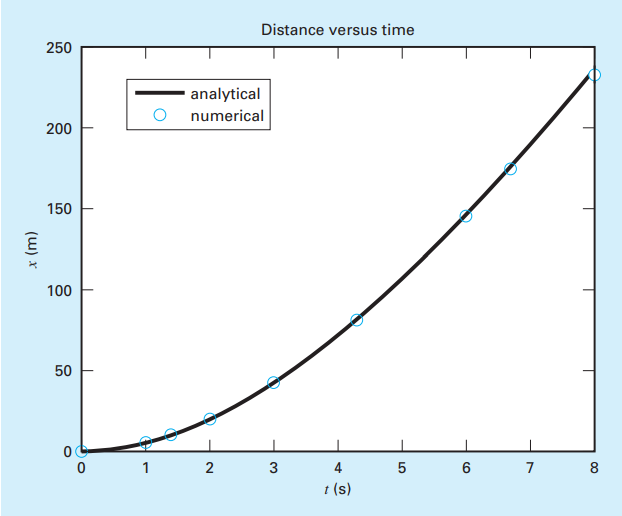
\includegraphics[scale=0.8]{fig_19_15}
   \caption{\textsf{Plot of distance versus time. The line was computed with the analytical solution, whereas the
   points were determined numerically with the cumtrapz function.}}\label{fig:fig_19_15}
\end{figure}

$$
\begin{aligned}
&\text { Segments }\\
&\begin{array}{cclll}
\text { (n) } & \text { Points } & \text { Name } & \text { Formula } & \text { Trunction Error } \\
\hline 2 & 1 & \text { Midpoint method } &(b-a) f\left(x_{1}\right) & (1 / 3) h^{3} f^{\prime \prime}(\xi)\\
3 & 2 & &(b-a) \frac{f\left(x_{1}\right)+f\left(x_{2}\right)}{2} & (3 / 4) h^{3} f^{\prime \prime}(\xi)\\
4 & 3 & &(b-a) \frac{2 f\left(x_{1}\right)-f\left(x_{2}\right)+2 f\left(x_{3}\right)}{3} & (14 / 45) h^{5} f^{(4)}(\xi) \\
5 & 4 & &(b-a) \frac{11 f\left(x_{1}\right)+f\left(x_{2}\right)+f\left(x_{3}\right)+11 f\left(x_{4}\right)}{24} & (95 / 144) h^{5} f^{(4)}(\xi)\\
6 & 5 & &(b-a) \frac{11 f\left(x_{1}\right)-14 f\left(x_{2}\right)+26 f\left(x_{3}\right)-14 f\left(x_{4}\right)+11 f\left(x_{5}\right)}{20} & (41 / 140) h^{7} f^{(6)}(\xi)\\
\hline
\end{array}
\end{aligned}
$$

\section{OPEN METHODS}

Recall from Fig. 19.6b that open integration formulas have limits that extend beyond the
range of the data. Table 19.4 summarizes the Newton-Cotes open integration formulas. The
formulas are expressed in the form of Eq. (19.13) so that the weighting factors are evident.
As with the closed versions, successive pairs of the formulas have the same-order error.
The even-segment-odd-point formulas are usually the methods of preference because they
require fewer points to attain the same accuracy as the odd-segment-even-point formulas.\\
The open formulas are not often used for definite integration. However, they have utility for analyzing improper integrals. In addition, they will have relevance to our discussion
of methods for solving ordinary differential equations in Chaps. 22 and 23.
\vspace{1cm}
\section{MULTIPLE INTEGRALS}
Multiple integrals are widely used in engineering and science. For example, a general
equation to compute the average of a two-dimensional function can be written as [recall
Eq. (19.7)]

\begin{equation}
    \tag{19.31}
\bar{f}=\frac{\int_{c}^{d}\left(\int_{a}^{b} f(x, y) d x\right)}{(d-c)(b-a)}
\end{equation}
The numerator is called a double integral.
The techniques discussed in this chapter (and Chap. 20) can be readily employed to evaluate multiple integrals. A simple example would be to take the double integral of a function over a rectangular area (Fig. 19.16).
Recall from calculus that such integrals can be computed as iterated integrals:
\begin{equation}
    \tag{19.32}
\int_{c}^{d}\left(\int_{a}^{b} f(x, y) d x\right) d y=\int_{a}^{b}\left(\int_{c}^{d} f(x, y) d y\right) d x
\end{equation}
Thus, the integral in one of the dimensions is evaluated first. The result of this first integration is integrated in the second dimension. Equation (19.32) states that the order of integration is not important.

\begin{figure}[H]
    \centering
    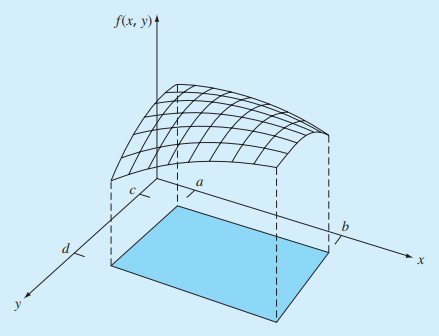
\includegraphics[scale=0.8]{fig_19_16}
   \caption{\textsf{Double integral as the area under the function surface.}}\label{fig:fig_19_16}
\end{figure}

A numerical double integral would be based on the same idea. First, methods such as
the composite trapezoidal or Simpson's rule would be applied in the first dimension with
each value of the second dimension held constant. Then the method would be applied to integrate the second dimension. The approach is illustrated in the following example.

\begin{exmp} \textbf{Using Double Integral to Determine Average Temperature}
    \noindent\textit{Problem Statement.} Suppose that the temperature of a rectangular heated plate is described by the following function:
	\begin{equation}
		T(x, y)=2 x y+2 x-x^{2}-2 y^{2}+72\nonumber
	\end{equation}
	If the plate is 8 m long (x dimension) and 6 m wide (y dimension), compute the average
temperature.
	
	\noindent \textbf{Solution.} First, let us merely use two-segment applications of the trapezoidal rule in each
	dimension. The temperatures at the necessary x and y values are depicted in Fig. 19.17.
	Note that a simple average of these values is 47.33. The function can also be evaluated analytically to yield a result of 58.66667.\\
	To make the same evaluation numerically, the trapezoidal rule is first implemented
along the x dimension for each y value. These values are then integrated along the y dimension to give the final result of 2544. Dividing this by the area yields the average temperature as $2544/(6\times8)=53$\\
Now we can apply a single-segment Simpson's 1/3 rule in the same fashion. This results
in an integral of 2816 and an average of 58.66667, which is exact. Why does this occur? Recall
that Simpson's 1/3 rule yielded perfect results for cubic polynomials. Since the highest-order
term in the function is second order, the same exact result occurs for the present case.

\begin{figure}[H]
    \centering
    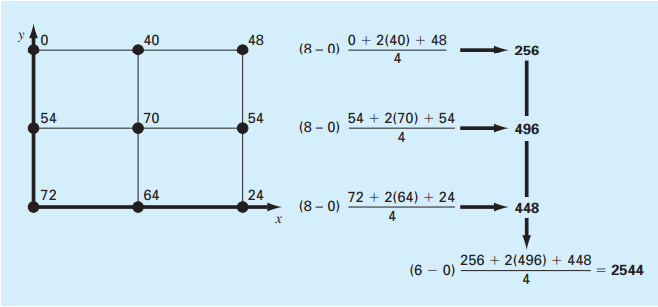
\includegraphics[scale=0.8]{fig_19_17}
   \caption{\textsf{Numerical evaluation of a double integral using the two-segment trapezoidal rule}}\label{fig:fig_19_17}
\end{figure}

For higher-order algebraic functions as well as transcendental functions, it would be
necessary to use composite applications to attain accurate integral estimates. In addition,
Chap. 20 introduces techniques that are more efficient than the Newton-Cotes formulas for
evaluating integrals of given functions. These often provide a superior means to implement
the numerical integrations for multiple integrals.

\end{exmp}

\subsection{MATLAB Functions: dblquad and triplequad}
MATLAB has functions to implement both double ($dblquad$) and triple ($triplequad$)
integration. A simple representation of the syntax for $dblquad$ is

\begin{lstlisting}[numbers=none]
	q = dblquad(fun, xmin, xmax, ymin, ymax, tol)
\end{lstlisting}

where $q$ is the double integral of the function fun over the ranges from xmin to xmax and ymin to ymax. If tol is not specified, a default tolerance of $1 \times 10^{-6}$ is used.

Here is an example of how this function can be used to compute the double integral evaluated in Example 19.7:

\begin{lstlisting}[numbers=none]
	>> q = dblquad(@(x,y) 2*x*y+2*x-x.^2-2*y.^2+72,0,8,0,6)
	q =
		2816
\end{lstlisting}

\section{CASE STUDY: COMPUTING WORK WITH NUMERICAL INTEGRATION}
\noindent \textbf{Background.} The calculation of work is an important component of many areas of
engineering and science. The general formula is

$$
		\text { Work }= \text { force } \times \text { distance }
		$$

		When you were introduced to this concept in high school physics, simple applications were
		presented using forces that remained constant throughout the displacement. For example,
		if a force of 10 N was used to pull a block a distance of 5 m, the work would be calculated
		as 50 J (1 joule = 1 N · m).\\
		Although such a simple computation is useful for introducing the concept, realistic
		problem settings are usually more complex. For example, suppose that the force varies during the course of the calculation. In such cases, the work equation is reexpressed as

		\begin{equation}
			\tag{19.33}
W=\int_{x_{0}}^{x_{n}} F(x) d x
\end{equation}
where $W=$ work $(\mathrm{J}), x_{0}$ and $x_{n}=$ the initial and final positions $(\mathrm{m})$, respectively, and $F(x)=$ a force that varies as a function of position (N). If $F(x)$ is easy to integrate, Eq. (19.33) can be evaluated analytically. However, in a realistic problem setting, the force might not be expressed in such a manner. In fact, when analyzing measured data, the force might be available only in tabular form. For such cases, numerical integration is the only viable option for the evaluation.

Further complexity is introduced if the angle between the force and the direction of movement also varies as a function of position (Fig. 19.18). The work equation can be modified further to account for this effect, as in
\begin{equation}
    \tag{19.34}
W=\int_{x_{0}}^{x_{n}} F(x) \cos [\theta(x)] d x
\end{equation}

Again, if $F(x)$ and $\theta(x)$ are simple functions, Eq. (19.34) might be solved analytically. However, as in Fig. 19.18, it is more likely that the functional relationship is complicated. For this situation, numerical methods provide the only alternative for determining the integral.
Suppose that you have to perform the computation for the situation depicted in Fig. 19.18. Although the figure shows the continuous values for $F(x)$ and $\theta(x)$, assume that, because of experimental constraints, you are provided with only discrete measurements at $x=5-\mathrm{m}$ intervals (Table 19.5). Use single- and composite versions of the trapezoidal rule and Simpson's $1 / 3$ and $3 / 8$ rules to compute work for these data.
\vspace{0.5cm}\\
\noindent \textbf{Solution.} The results of the analysis are summarized in Table 19.6. A percent relative error $\varepsilon_{t}$ was computed in reference to a true value of the integral of $129.52$ that was estimated on the basis of values taken from Fig. $19.18$ at 1 -m intervals.

The results are interesting because the most accurate outcome occurs for the simple two-segment trapezoidal rule. More refined estimates using more segments, as well as Simpson's rules, yield less accurate results.

The reason for this apparently counterintuitive result is that the coarse spacing of the points is not adequate to capture the variations of the forces and angles. This is particularly

\begin{figure}[H]
    \centering
    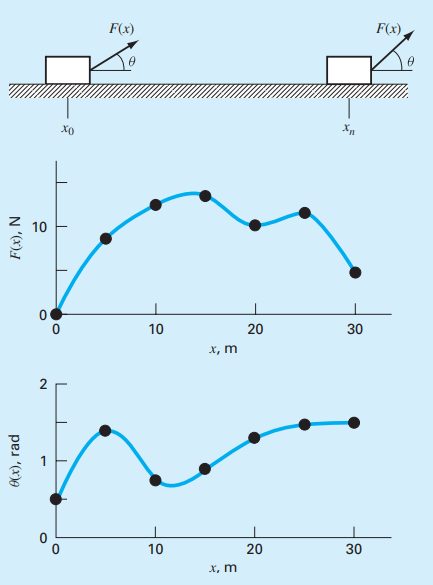
\includegraphics[scale=0.8]{fig_19_18}
   \caption{\textsf{The case of a variable force acting on a block. For this case the angle, as well as the
   magnitude, of the force varies.}}\label{fig:fig_19_18}
\end{figure}

\textit{TABLE 19.5} Data for force $F(x)$ and angle $\theta(x)$ as a function of position $x$.
\begin{center}
\begin{tabular}{cccc}
\hline $\boldsymbol{x}, \mathbf{m}$ & $\boldsymbol{F}(\boldsymbol{x}), \mathbf{N}$ & $\boldsymbol{\theta}$, rad & $\boldsymbol{F}(\boldsymbol{x}) \cos \boldsymbol{\theta}$ \\
\hline 0 & $0.0$ & $0.50$ & $0.0000$ \\
5 & $9.0$ & $1.40$ & $1.5297$ \\
10 & $13.0$ & $0.75$ & $9.5120$ \\
15 & $14.0$ & $0.90$ & $8.7025$ \\
20 & $10.5$ & $1.30$ & $2.8087$ \\
25 & $12.0$ & $1.48$ & $1.0881$ \\
30 & $5.0$ & $1.50$ & $0.3537$ \\
\hline
\end{tabular}
\end{center}

\textit{TABLE 19.6} Estimates of work calculated using the trapezoidal rule and Simpson's rules. The percent relative error $\varepsilon_{t}$ as computed in reference to a true value of the integral $(129.52 \mathrm{~Pa})$ that was estimated on the basis of values at $1-\mathrm{m}$ intervals.

\begin{center}
\begin{tabular}{lcrr}
\hline Technique & Segments & Work & $\boldsymbol{\varepsilon}_{\boldsymbol{t}}\%{}$ \\
\hline Trapezoidal rule & 1 & $5.31$ & $95.9$ \\
& 2 & $133.19$ & $2.84$ \\
& 3 & $124.98$ & $3.51$ \\
& 6 & $119.09$ & $8.05$ \\
Simpson's $1 / 3$ rule & 2 & $175.82$ & $35.75$ \\
& 6 & $117.13$ & $9.57$ \\
Simpson's $3 / 8$ rule & 3 & $139.93$ & $8.04$ \\
\hline
\end{tabular}
\end{center}

\begin{figure}[H]
    \centering
    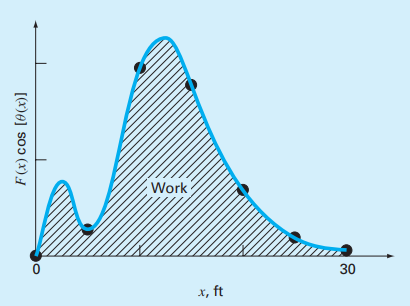
\includegraphics[scale=0.8]{fig_19_19}
   \caption{\textsf{A continuous plot of F(x) cos [$\theta$(x)] versus position with the seven discrete points used to develop
   the numerical integration estimates in Table 19.6. Notice how the use of seven points to
   characterize this continuously varying function misses two peaks at x = 2.5 and 12.5 m.}}\label{fig:fig_19_19}
\end{figure}

evident in Fig. 19.19, where we have plotted the continuous curve for the product of F(x)
and cos [$\theta$(x)]. Notice how the use of seven points to characterize the continuously varying
function misses the two peaks at x = 2.5 and 12.5 m. The omission of these two points effectively limits the accuracy of the numerical integration estimates in Table 19.6. The fact
that the two-segment trapezoidal rule yields the most accurate result is due to the chance
positioning of the points for this particular problem (Fig. 19.20).\\
The conclusion to be drawn from Fig. 19.20 is that an adequate number of measurements must be made to accurately compute integrals. For the present case, if data were
available at F(2.5) cos [$\theta$(2.5)] = 3.9007 and F(12.5) cos [$\theta$(12.5)] = 11.3940, we could

\begin{figure}[H]
    \centering
    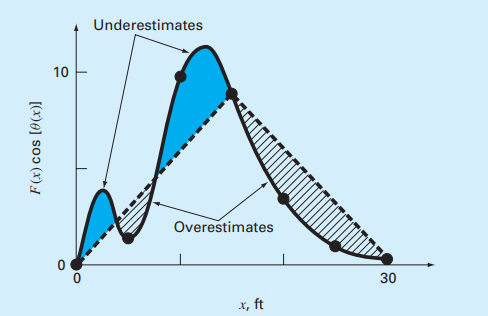
\includegraphics[scale=0.8]{fig_19_20}
   \caption{\textsf{Graphical depiction of why the two-segment trapezoidal rule yields a good estimate of the
   integral for this particular case. By chance, the use of two trapezoids happens to lead to an
   even balance between positive and negative errors.}}\label{fig:fig_19_20}
\end{figure}

determine an improved integral estimate. For example, using the MATLAB trapz function, we could compute

\begin{lstlisting}[numbers=none]
>> x=[0 2.5 5 10 12.5 15 20 25 30];
>> y=[0 3.9007 1.5297 9.5120 11.3940 8.7025 2.8087 ...
1.0881 0.3537];
>> trapz(x,y)
ans =
132.6458
\end{lstlisting}

Including the two additional points yields an improved integral estimate of 132.6458
($\epsilon\textsubscript{t}$ = 2.16\%{}). Thus, the inclusion of the additional data incorporates the peaks that were
missed previously and, as a consequence, lead to better results.
\vspace{1cm}
\section{PROBLEMS}

\noindent\textit{19.1} Derive Eq. (19.4) by integrating Eq. (19.3).
\\\noindent\textit{19.2} Evaluate the following integral:
$$\int_{0}^{4}\left(1-e^{-x}\right) d x$$
(a) analytically, (b) single application of the trapezoidal rule,
(c) composite trapezoidal rule with n = 2 and 4, (d) single
application of Simpson's 1/3 rule, (e) composite Simpson's
1/3 rule with n = 4, (f) Simpson's 3/8 rule, and (g) composite Simpson's rule, with n = 5. For each of the numerical
estimates (b) through (g), determine the true percent relative
error based on (a).
\\\noindent\textit{19.3} Evaluate the following integral:
$$\int_{0}^{\pi / 2}(8+4 \cos x) d x$$
(a) analytically, (b) single application of the trapezoidal rule,
(c) composite trapezoidal rule with n = 2 and 4, (d) single
application of Simpson's 1/3 rule, (e) composite Simpson's
1/3 rule with n = 4, (f) Simpson's 3/8 rule, and (g) composite Simpson's rule, with n = 5. For each of the numerical
estimates (b) through (g), determine the true percent relative
error based on (a).
\\\noindent\textit{19.4} Evaluate the following integral:
$$\int_{-2}^{4}\left(1-x-4 x^{3}+2 x^{5}\right) d x$$
(a) analytically, (b) single application of the trapezoidal rule,
(c) composite trapezoidal rule with n = 2 and 4, (d)single application of Simpson's 1/3 rule, (e) Simpson's 3/8 rule, and
(f)Boole's rule. For each of the numerical estimates(b)through
(f), determine the true percent relative error based on (a).
\\\noindent\textit{19.5} The function
$$
f(x)=e^{-x}
$$
can be used to generate the following table of unequally spaced data:
\begin{center}
\begin{tabular}{llllllll}
\hline $\boldsymbol{x}$ & 0 & $0.1$ & $0.3$ & $0.5$ & $0.7$ & $0.95$ & $1.2$ \\
$\boldsymbol{f}(\boldsymbol{x})$ & 1 & $0.9048$ & $0.7408$ & $0.6065$ & $0.4966$ & $0.3867$ & $0.3012$ \\
\hline
\end{tabular}
\end{center}

Evaluate the integral from a = 0 to b = 0.6 using (a) analytical means, (b) the trapezoidal rule, and (c) a combination
of the trapezoidal and Simpson's rules wherever possible to
attain the highest accuracy. For (b) and (c), compute the true
percent relative error.

\noindent\textit{19.6} Evaluate the double integral
$$\int_{-2}^{2} \int_{0}^{4}\left(x^{2}-3 y^{2}+x y^{3}\right) d x d y$$
(a) analytically, (b) using the composite trapezoidal rule
with n = 2, and (c) using single applications of Simpson's
1/3 rule. For (b) and (c), compute the percent relative error.\\
\\\noindent\textit{19.7} Evaluate the triple integral
$$
\int_{-4}^{4} \int_{0}^{6} \int_{-1}^{3}\left(x^{3}-2 y z\right) d x d y d z
$$
(a) analytically, and (b) using single applications of Simpson's $1 / 3$ rule. For (b), compute the true percent relative error.\\
\\\noindent\textit{19.8} Determine the distance traveled from the following velocity data:

\begin{center}
\begin{tabular}{llllllllllr}
\hline $\boldsymbol{t}$ & 1 & 2 & $3.25$ & $4.5$ & 6 & 7 & 8 & $8.5$ & 9 & 10 \\
$\boldsymbol{v}$ & 5 & 6 & $5.5$ & 7 & $8.5$ & 8 & 6 & 7 & 7 & 5 \\
\hline
\end{tabular}
\end{center}

(a) Use the trapezoidal rule. In addition, determine the average velocity.
(b) Fit the data with a cubic equation using polynomial
regression. Integrate the cubic equation to determine the
distance.

\noindent\textit{19.9}




\end{document}

$s\textsubscript{i}$

\begin{equation}
    \tag{19.3} \nonumber
    -
\end{equation}

\begin{lstlisting}[numbers=none]
\end{lstlisting}

\section{INTRODUCTION TO SPLINES}
\subsection{End Conditions}

\begin{figure}[H]
    \centering
    \includegraphics[scale=0.8]{fig_19_}
   \caption{\textsf{}}\label{fig:fig_19_}
\end{figure}

\begin{exmp} \textbf{First-Order Splines}
    \noindent\textit{Problem Statement.}
    \noindent \textbf{Solution.}
\end{exmp}